\documentclass{beamer}
\usepackage{ dsfont }
\usepackage[utf8]{inputenc}
\usepackage[english]{babel}
\setbeamersize{text margin left=10pt, text margin right=10pt} %new code
\usepackage{graphicx}
\usepackage{float}
\usepackage{subcaption}
\usepackage{minted}
\usefonttheme{professionalfonts} % using non standard fonts for beamer
\setbeamerfont{frametitle}{series=\bfseries}
\usepackage{animate}
\usepackage{movie15}
\usepackage{breqn, bm}
\usepackage{amsmath}
\usepackage[skins]{tcolorbox}
\usepackage{subcaption}

\definecolor{notgreen}{RGB}{255,127,0}
\definecolor{green}{RGB}{49,150,3}
\setbeamerfont{headline}{size=\small}


%----------------------------------------------------------------------------------------
%	 Package
%----------------------------------------------------------------------------------------
\usepackage{color}
\usepackage{url}
\beamertemplatenavigationsymbolsempty
\definecolor{cadmiumred}{rgb}{0.8, 0.8, 0.8}

%----------------------------------------------------------------------------------------
%	 Presentation settings
%----------------------------------------------------------------------------------------

\usetheme{default}
\usecolortheme{default}

\setbeamertemplate{itemize items}[triangle] 
\setbeamertemplate{enumerate items}[default]
 
\title[Variational Drop Out]{
	MSU Deep Learning Course\\ 
	\vspace{1cm}
	\textbf{\textcolor{black}{Image Captioning}}}

\author{Ashuha Arseniy$^{1, 2}$}
\institute[Bayesgroup, MIPT]{
	Bayesian Research Group$^1$, MIPT$^2$\\
	
	\medskip
	
\includegraphics[scale=0.5]{./img/logo} 
\includegraphics[scale=0.12]{./img/mipt}
	
	\href{ars-ashuha.ru/slides}{ars-ashuha.ru/slides}}

\date{\today}

\newcommand{\Expect}{\mathsf{E}}
\newcommand{\MExpect}{\mathsf{M}}
\newcommand{\cov}{\mathsf{cov}}
\setbeamertemplate{section in toc}[circle]

\addtobeamertemplate{navigation symbols}{}{%
	\usebeamerfont{footline}%
	\usebeamercolor[fg]{footline}%
	\hspace{1em}%
	\insertframenumber/\inserttotalframenumber
}


\begin{document}
\begin{frame}
	\titlepage 
\end{frame}

\begin{frame}{Motivation}
	
	\begin{itemize}
		  \item  What do we want?
		
			 \begin{center}
				  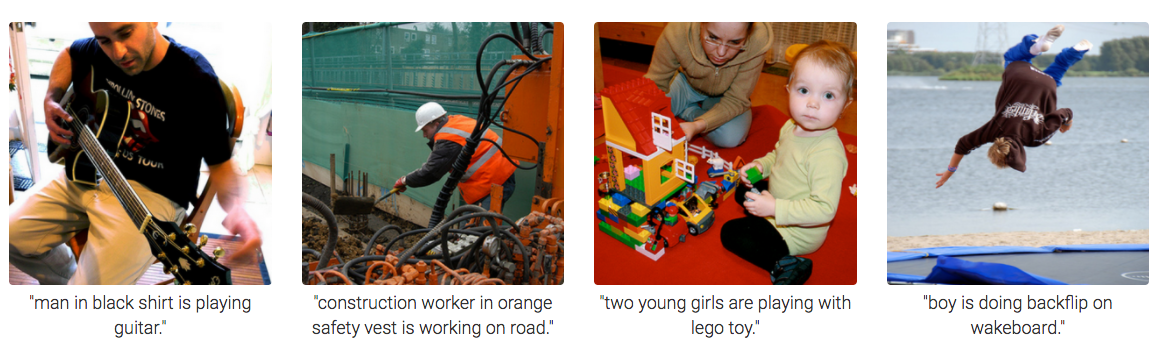
\includegraphics[scale=0.25]{img/ic} 
			\end{center}
			
			\item  Applications
		
		\begin{figure}[htbp]
			\centering
			 \begin{subfigure}[b]{0.25\textwidth}
				
				
\includegraphics[width=\textwidth]{img/wr}
				
				\caption{Your's example}
			\end{subfigure}
			 \begin{subfigure}[b]{0.25\textwidth}
				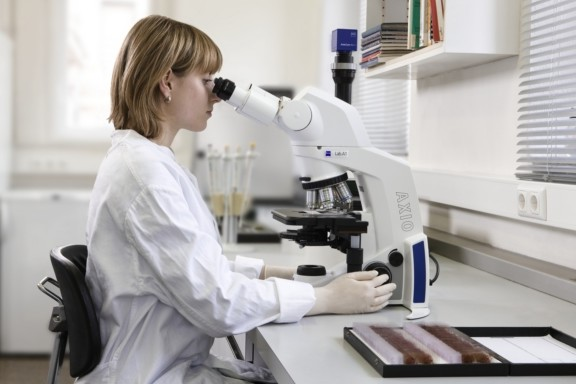
\includegraphics[width=\textwidth]{img/mic}
				\caption{Medicine}
			\end{subfigure}
			 \begin{subfigure}[b]{0.25\textwidth}
				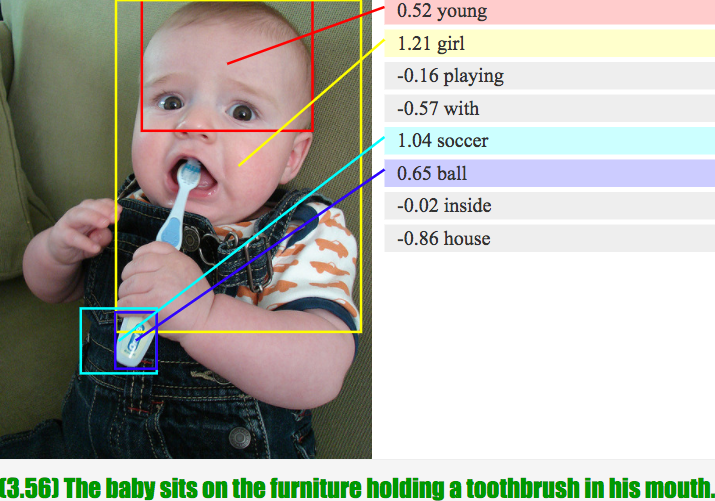
\includegraphics[width=\textwidth]{img/baby}
				\caption{Search engine}
			\end{subfigure}

		\end{figure}
			
			 \href{http://cs.stanford.edu/people/karpathy/deepimagesent/rankingdemo/}{http://cs.stanford.edu/people/karpathy/deepimagesent/rankingdemo/}
	\end{itemize}

\end{frame}

\begin{frame}{Recurrent Nets Recap}
	\begin{itemize}
		\item We want to process a number of inputs, each item is a sequence 
		
		\begin{center}
			 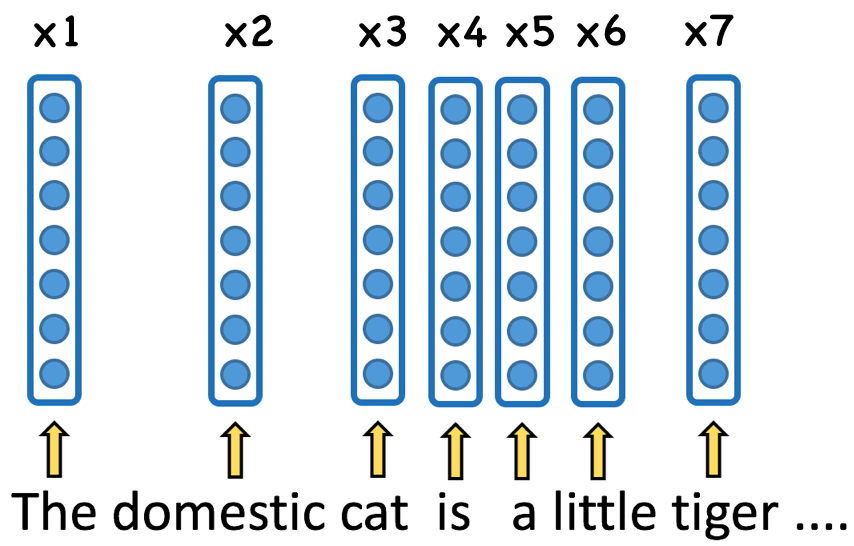
\includegraphics[scale=0.13]{img/emb}~~
			 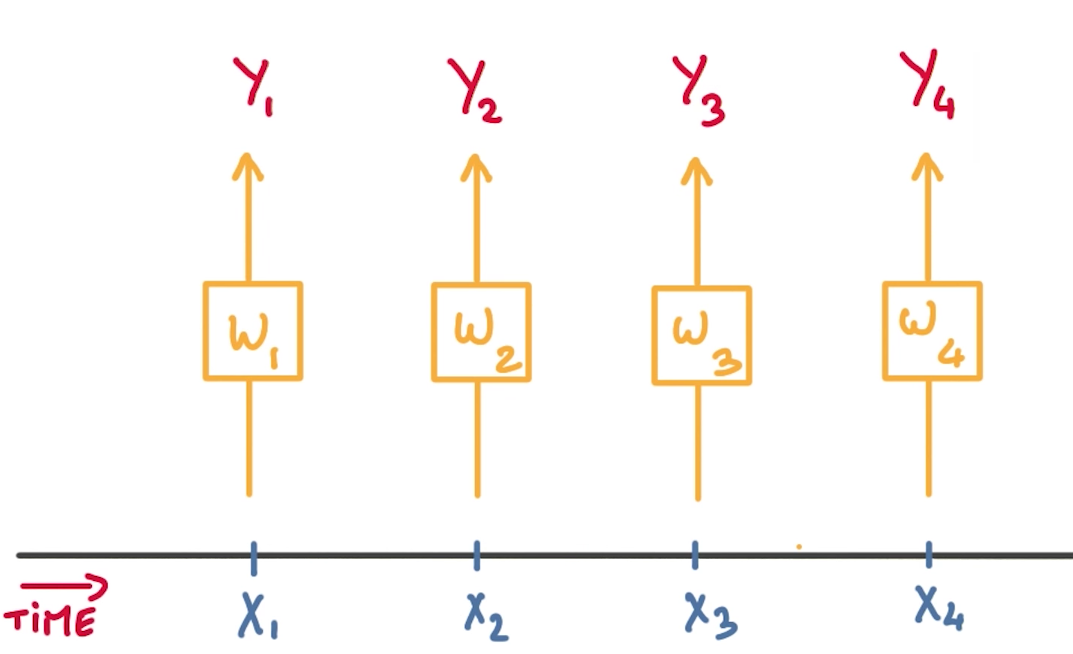
\includegraphics[scale=0.11]{img/rec}
		\end{center}
		
		\item  We will add recurrent connections and memory control options
		\begin{center}
			 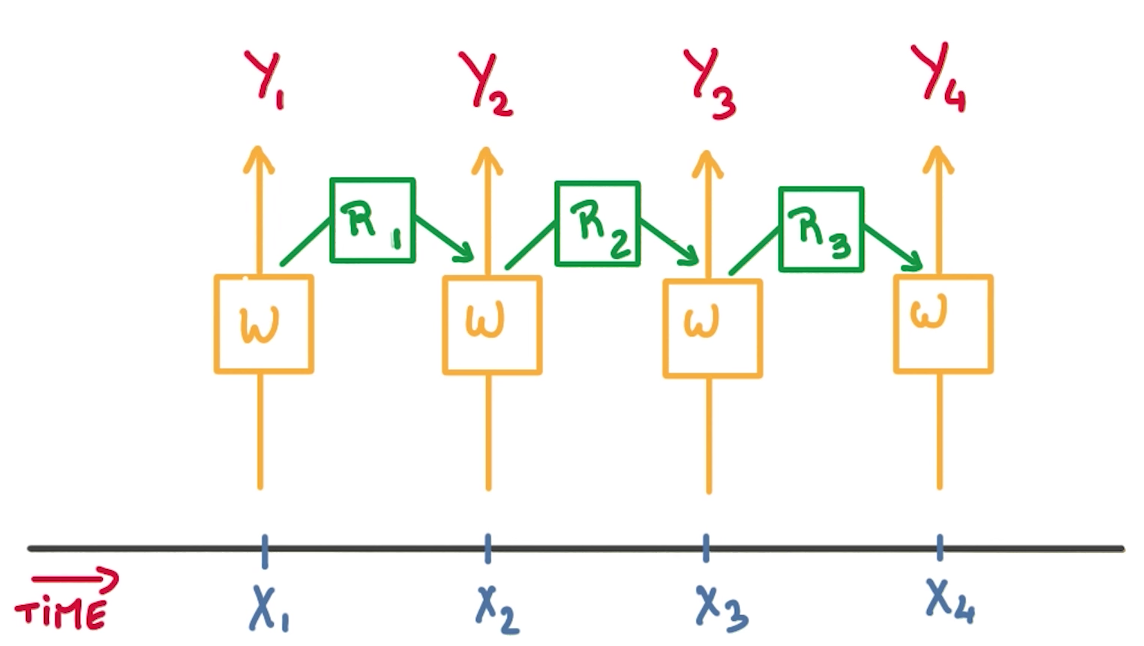
\includegraphics[scale=0.13]{img/rec2}
			 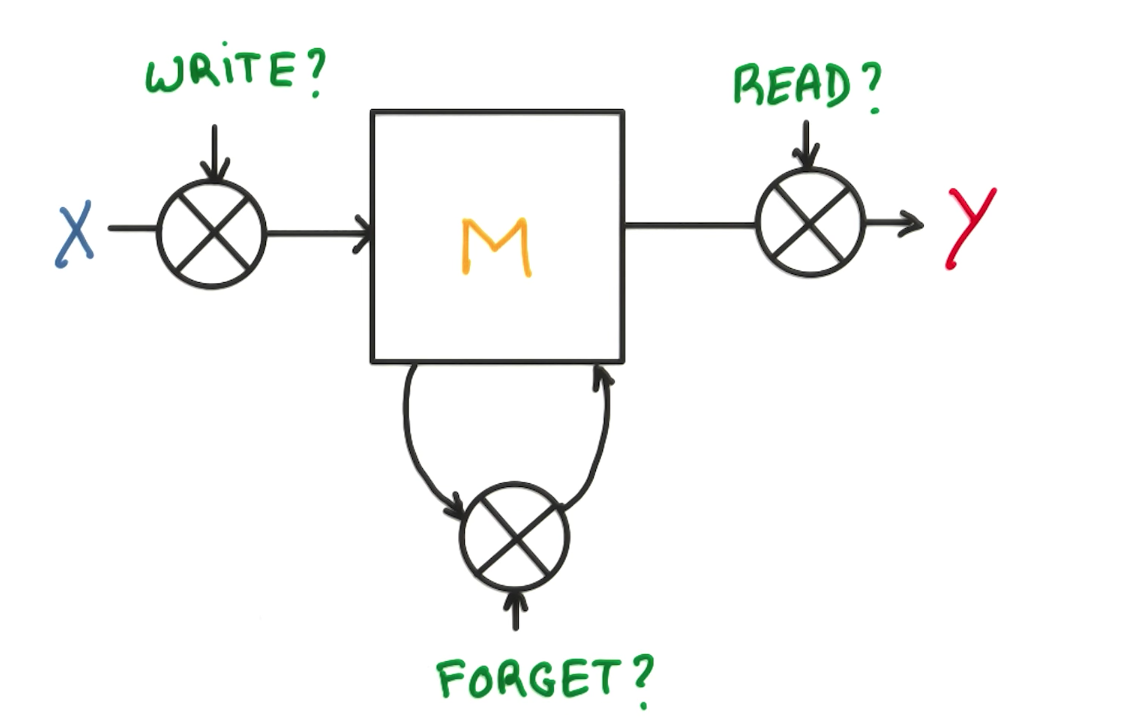
\includegraphics[scale=0.1]{img/lstm}
		\end{center}
	\item  \texttt{lasagne.layers.EmbeddingLayer, lasagne.layers.LSTMLayer}
	\end{itemize}
\end{frame}

\begin{frame}{Text Generative Model}
	\begin{itemize}
		\item   What is a text generative model?
			   $$p(w_{n+1}|w_1, \dots, w_n; \theta)$$
		\item     Let's specify dimensions:
		\begin{itemize}
			\item[$-$]     $p(w_{n+1}).shape$      is vocabulary size
			\item[$-$]    $w_i.shape$     is embedding size
			\item[$-$]     $\theta.shape$     has shape like parameters
		\end{itemize}
		\item     How can we define this function?    RNN!
		   $$p(w_{n+1}|w_1, \dots, w_n; \theta) = p(w_{n+1}|w_n, hiden_{n-1}; \theta)$$
	\end{itemize}
	 	   \begin{tcolorbox}[enhanced,size=fbox,fontupper=\large\bfseries, colback=black!80, colframe=black!80]
	 		\begin{center}
	 			\text{\textcolor{white}{But, there are several technical problems to apply it}}
	 		\end{center}
	 	\end{tcolorbox}
	 	\begin{itemize}
	 		  \item How would you to construct a batch?
	 		  \item How to define loss functions?
	 		  \item How to calculate soft-max over millions point? 
	 	\end{itemize}
\end{frame}

\begin{frame}{Tech Details and General Scheme}
	\begin{center}
			\onslide<1>{\centering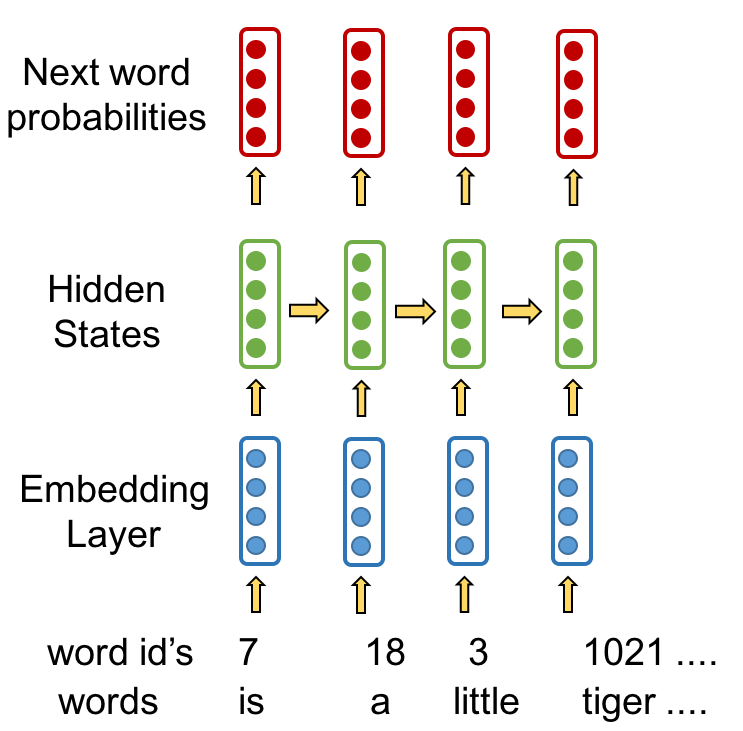
\includegraphics[scale=0.5]{img/gensch}}
			
			\vspace{-6cm}\onslide<2>{\centering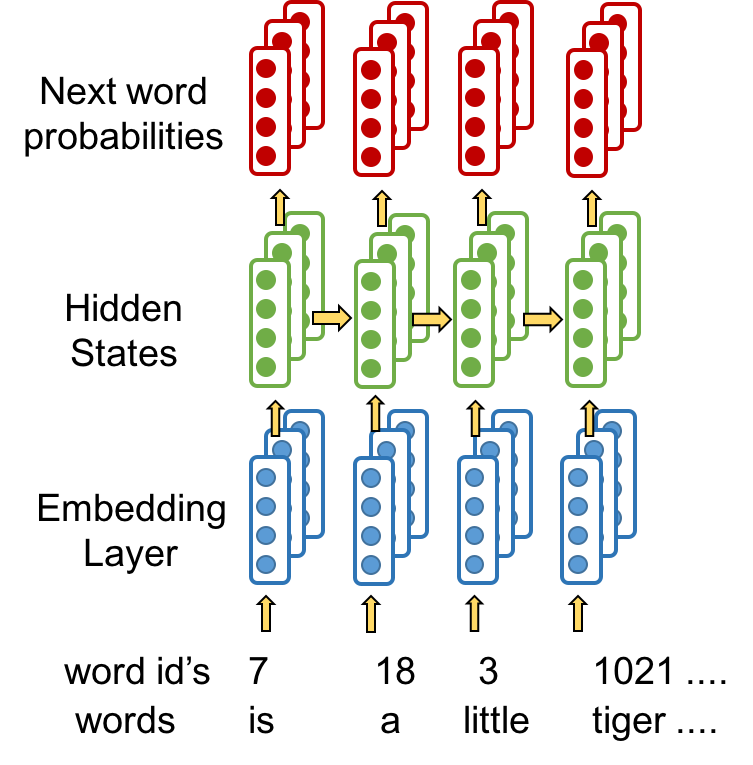
\includegraphics[scale=0.5]{img/senschb}}
			
			\vspace{-7cm} \onslide<3>{\centering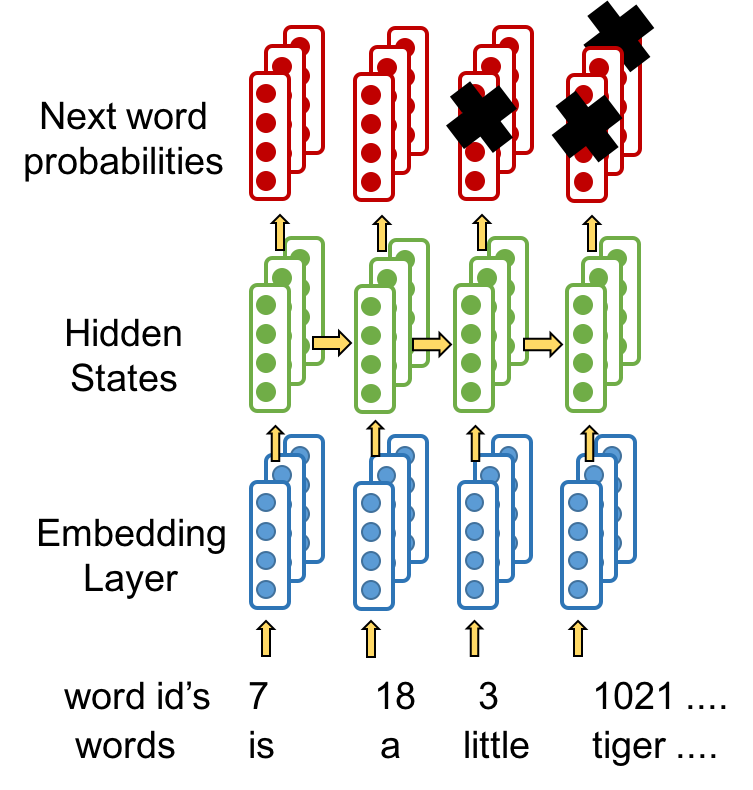
\includegraphics[scale=0.5]{img/genschmask}}
	\end{center}
\end{frame}

\begin{frame}{Convolution Net Recap}
	\begin{itemize}
		\item   Convolution (lower number of parameters cmp with fully connected)  
		\item   Convolution and Convolution Neural Net
				\begin{center}
					  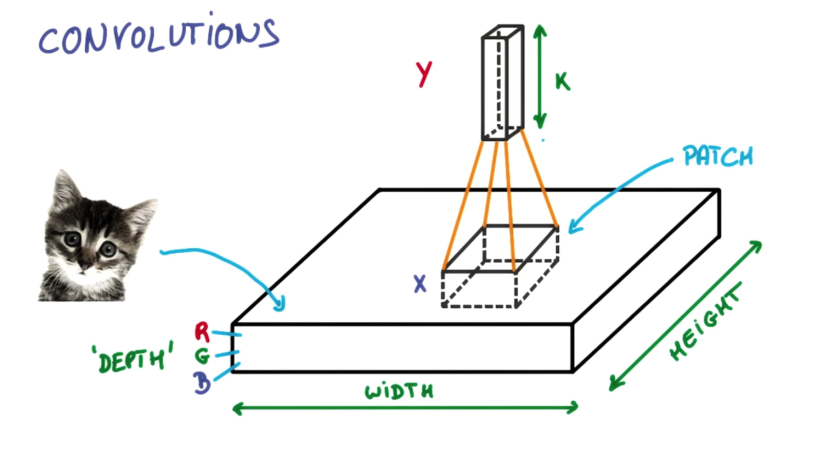
\includegraphics[scale=0.17]{img/cnn2}~~
					  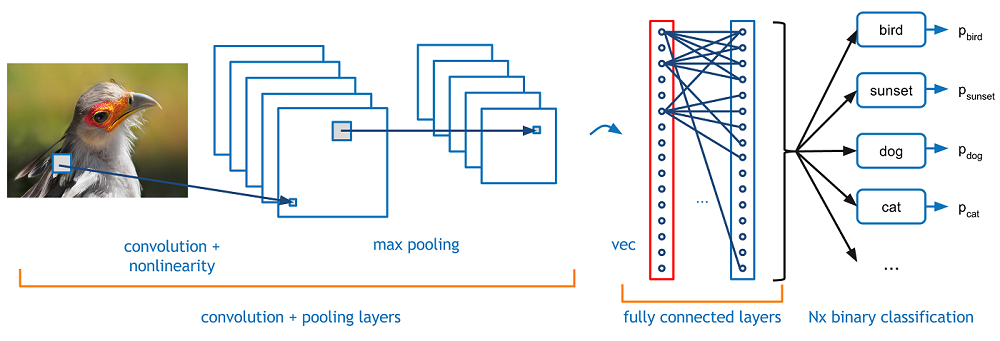
\includegraphics[scale=0.35]{img/cnn5}
				\end{center}
		
		\item  Modern Architecture (VGG16)
				\begin{center}
					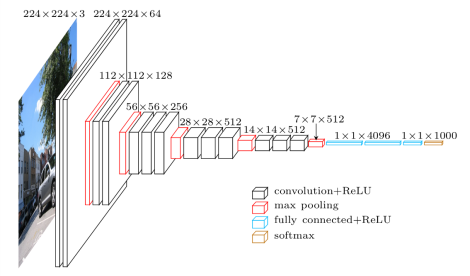
\includegraphics[scale=0.2]{img/cnn3}
				\end{center}
	\end{itemize}
\end{frame}

\begin{frame}{Condition Text Generative Model}
	\begin{itemize}
		\item   How to build image captioning Neural Nets?
			 \begin{center}
				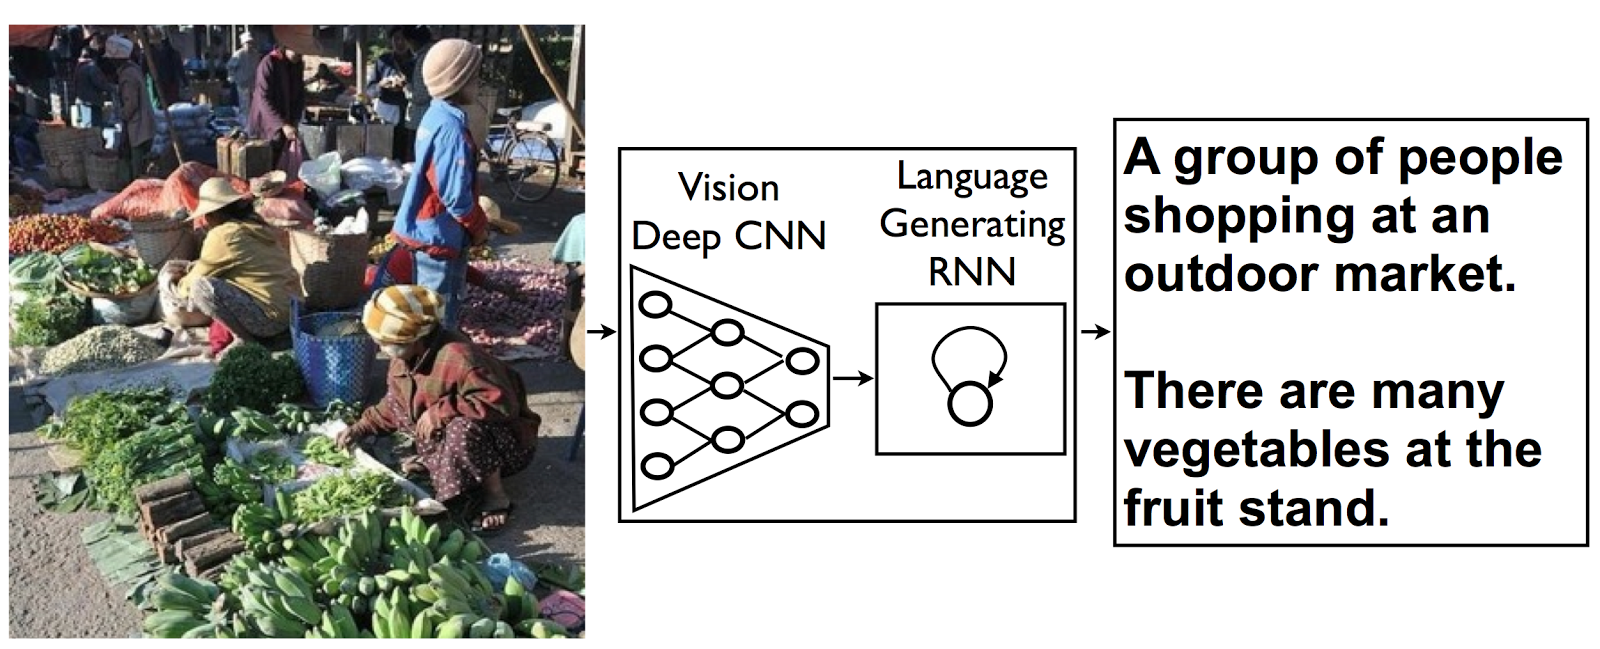
\includegraphics[scale=0.1]{img/googlernncnn.png}
			\end{center}
		\item  Another useful thinks?
					 \begin{center}
						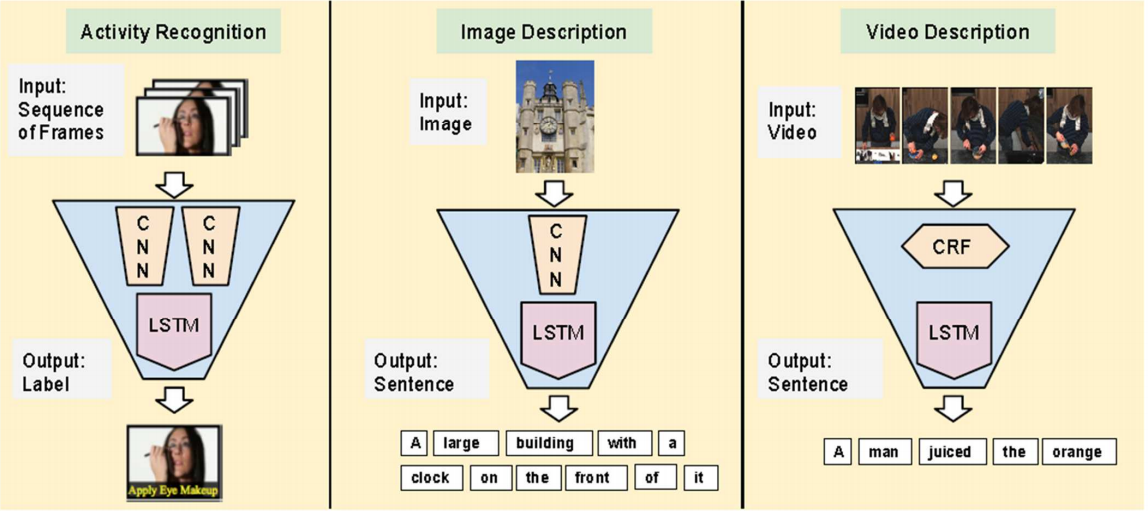
\includegraphics[scale=0.17]{img/im2txt}
					\end{center}
	\end{itemize}
	
		 	 \begin{tcolorbox}[enhanced,size=fbox,fontupper=\large\bfseries, colback=black!80, colframe=black!80]
		 		\begin{center}
		 			\text{\textcolor{white}{But, extremely complex to train}}
		 		\end{center}
		 	\end{tcolorbox}

	
	 \href{http://cs.stanford.edu/people/karpathy/cvpr2015.pdf}{http://cs.stanford.edu/people/karpathy/cvpr2015.pdf}
\end{frame}

\begin{frame}[fragile]{Code should be like this}
	 
\begin{minted}{python}
sentences = T.imatrix()# word ids
image_vec = T.matrix() # image features
sentence_mask = T.neq(sentences, PAD_ix)
\end{minted}
 
\begin{minted}{python}
words = InputLayer((None, None), sentences)
masks = InputLayer((None, None), sentence_mask)
words_emb = EmbeddingLayer(words, n_tokens, EMBED_SIZE)
\end{minted}
 
\begin{minted}{python}
image_fea = InputLayer((None, CNN_FEATURE_SIZE), image_vec)
image_emb = DropoutLayer(image_fea, 0.5)
image_emb = DenseLayer(image_emb, LSTM_UNITS)
\end{minted}
 
\begin{minted}{python}
decoder = LSTMLayer(
	words_emb, num_units=LSTM_UNITS,
	cell_init=image_emb, mask_input=mask)
\end{minted}
 
\begin{minted}{python}
decoder = Reshape (...)
loss = categorical_cross_enrtopy (...)
\end{minted}
\end{frame}

\begin{frame}{AWS Educate}
	\begin{itemize}
		\item  Training is extremely hard, so you should use pre-train models
		\item  If it's still hard, let's use gpu
				\begin{center}
					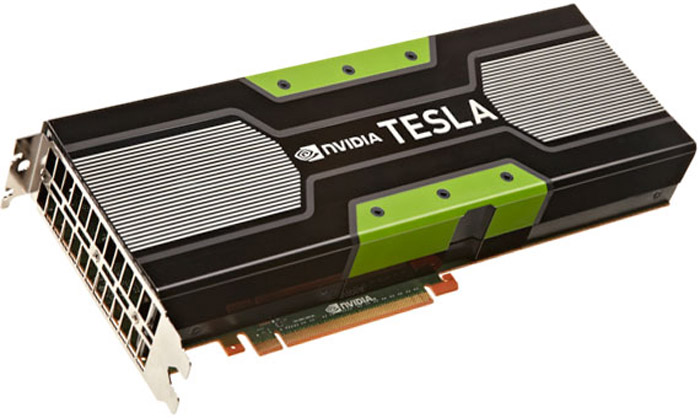
\includegraphics[scale=0.3]{img/tesla}
				\end{center}
		\item  But gpu is a little bit expensive
		\item  AWS Educate give 100\$ grand for all MSU students $\approx$ 160 hours
		\item  You need only MSU email
		\item  You can rent GPU server on Amazon WS free using this money!!!
	\end{itemize}
	 \href{https://aws.amazon.com/ru/education/awseducate/}{https://aws.amazon.com/ru/education/awseducate/}
\end{frame}

\begin{frame}{Go To Break}
		\begin{center}
			
\includegraphics[scale=0.25]{img/cof.png}
		\end{center}
\end{frame}


\begin{frame}{Image Captioning Seminar}
	
	 \begin{center}
				  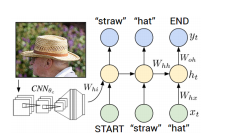
\includegraphics[scale=1.0]{img/ic3}
				
				  \href{http://mybinder.org/repo/ars-ashuha/caption_binder}{\textcolor{red}{http://mybinder.org/repo/ars-ashuha/caption\_binder}}
	\end{center}
\end{frame}
\end{document}

